\documentclass{article}
\usepackage{tikz}
\usetikzlibrary{shapes.geometric, arrows}

\tikzstyle{startstop} = [rectangle, rounded corners, minimum width=3cm, minimum height=1cm, text centered, draw=black, fill=red!30]
\tikzstyle{process} = [rectangle, minimum width=3cm, minimum height=1cm, text centered, draw=black, fill=orange!30]
\tikzstyle{decision} = [diamond, minimum width=3cm, minimum height=1cm, text centered, draw=black, fill=green!30]

\tikzstyle{arrow} = [thick,->,>=stealth]

\begin{document}

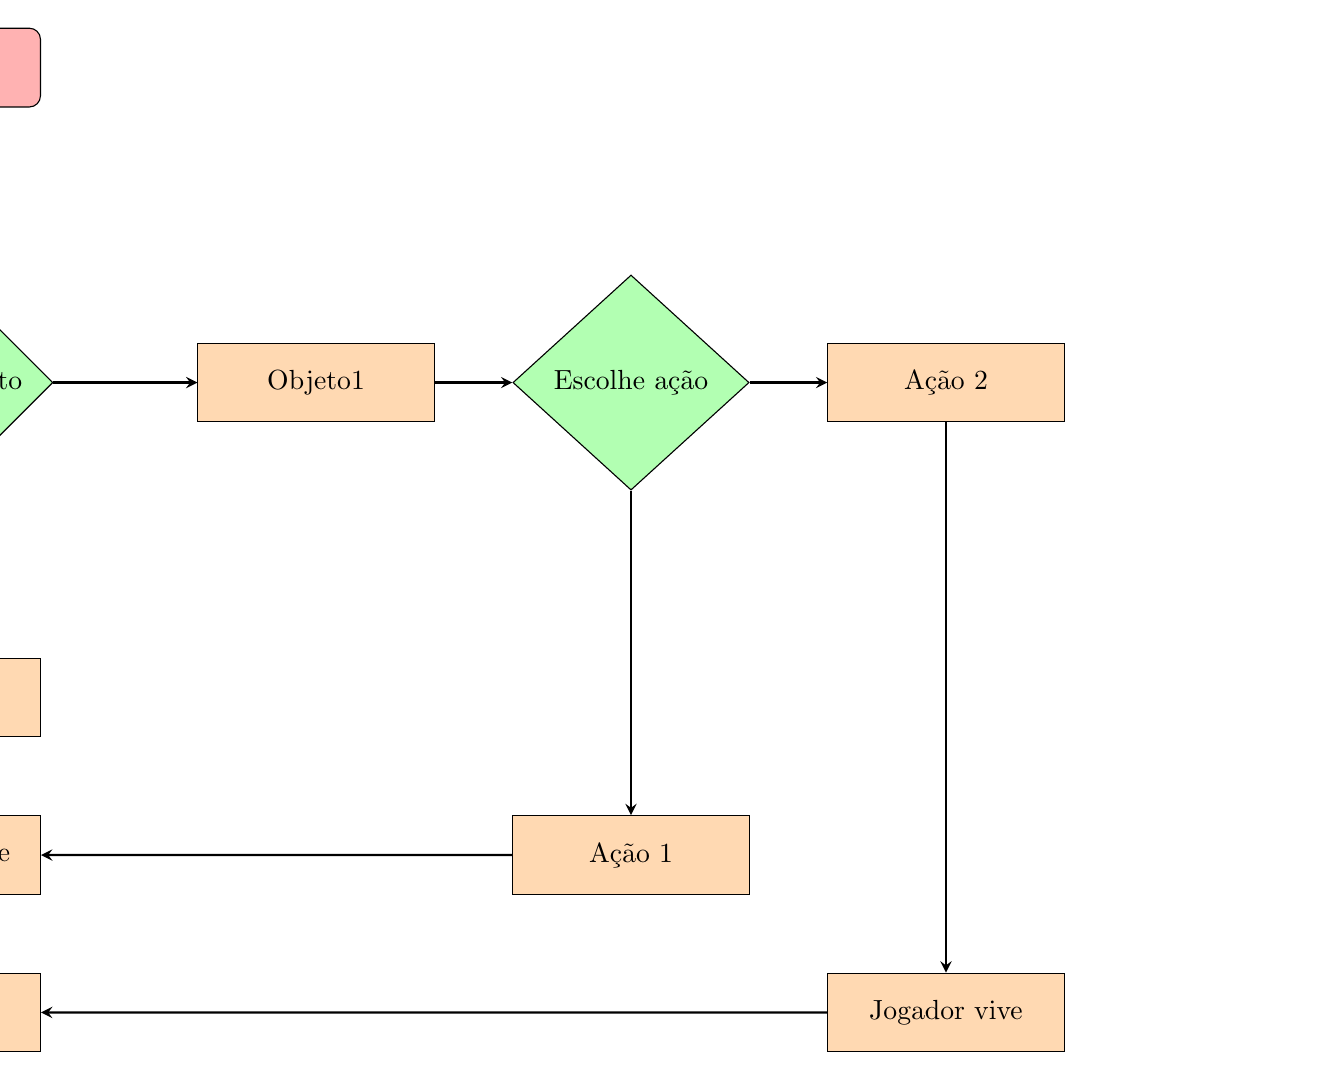
\begin{tikzpicture}[node distance=2cm]
\hspace{-3cm}

\node (start) [startstop] {Início};
\node (choice1) [decision, below of=start, yshift=-2cm] {Escolhe o objeto};
\node (veneno) [process, right of=choice1, xshift=3cm] {Objeto1};
\node (açao) [decision, right of=veneno, xshift=2cm] {Escolhe ação};
\node (bebe) [process, below of=açao, yshift=-4cm] {Ação 1};
\node (quebra) [process, right of=açao, xshift=2cm] {Ação 2};
\node (vive) [process, below of=quebra, yshift=-6cm] {Jogador vive};
\node (suco) [process, below of=choice1, yshift=-2cm] {Objeto 2};
\node (death) [process, below of=suco, yshift=0cm] {Jogador morre};
\node (fim) [process, below of=death, yshift=0cm] {Fim};

\draw [arrow] (start) -- (choice1);
\draw [arrow] (choice1) -- (veneno);
\draw [arrow] (choice1) -- (suco);
\draw [arrow] (veneno) -- (açao);
\draw [arrow] (açao) -- (quebra);
\draw [arrow] (quebra) -- (vive);
\draw [arrow] (vive) -- (fim);
\draw [arrow] (suco) -- (death);
\draw [arrow] (death) -- (fim);
\draw [arrow] (bebe) -- (death);
\draw [arrow] (açao) -- (bebe);

\end{tikzpicture}
